% ============================================================
% Praktická část, bod 2: Návrh architektury, databázového modelu
% a uživatelského rozhraní aplikace
% Návrh se porovnává s doporučeními z teoretické části
% (kapitoly kap:uzivatelske-rozhrani a kap:principy-db).
% ============================================================
\chapter{Návrh architektury, databázového modelu a~uživatelského rozhraní aplikace}\label{kap:architektura}

Tato kapitola popisuje návrh aplikace na základě požadavků z~kapitoly~\ref{kap:analyza-workflow}. Nejprve představuje aplikaci jako celek, její architekturu a~strukturu zdrojového kódu. Potom popisuje databázový model a~porovnává ho s~principy návrhu z~kapitoly~\ref{kap:principy-db}. Na konci porovnává uživatelské rozhraní se zásadami z~kapitoly~\ref{kap:uzivatelske-rozhrani}. Jak jsou jednotlivé funkce implementovány, popisují kapitoly~\ref{kap:funkce} a~\ref{kap:dokumenty}.

% delší názvy souborů a identifikátorů v textu se lépe zalomí
\begingroup\sloppy
% ============================================================
% Celkový popis aplikace (zkrácená verze; úplný popis je v dokumentaci
% aplikace: docs/01-popis-aplikace.md v repozitáři)
% ============================================================
\section{Celkový popis aplikace}\label{sec:popis-aplikace}

Výsledkem praktické části práce je aplikace \textbf{BusinessManager}, informační systém pro evidenci servisních zakázek navržený pro malou servisní firmu zabývající se opravami elektromotorů a~dalších technických zařízení. Aplikace sdružuje na jednom místě vše, co se ve firmě dříve evidovalo odděleně v~papírových formulářích, tabulkách aplikace Excel a~složkách s~fotografiemi: zákazníky, jejich zařízení, průběh opravy, provedené práce, použitý materiál a~z~nich vytvářené zakázkové listy, cenové nabídky a~faktury. Podrobný popis aplikace pro uživatele je součástí její dokumentace\footnote{\url{https://github.com/MajkyyQ/BusinessManager/blob/main/docs/01-popis-aplikace.md}}.

\subsection{Hlavní myšlenky aplikace}\label{sec:popis-aplikace-problem}

Analýza procesů (kapitola~\ref{kap:analyza-procesu}) ukázala, že se stejné údaje ve firmě opakovaně přepisovaly mezi dokumenty, stav zakázek a~historie oprav se dohledávaly pracně a~součty, DPH i~číslování dokladů se počítaly ručně. Aplikace na to odpovídá dvěma myšlenkami:

\begin{itemize}
\item \textbf{Každý údaj se zadává pouze jednou.} Zákazník, zařízení nebo položka materiálu se zapíší, když se poprvé objeví, a~dále se na ně jen odkazuje. Nabídku nebo fakturu aplikace sestaví sama z~prací a~materiálu evidovaných u~zakázky a~doplní údaje o~zákazníkovi a~o~firmě.
\item \textbf{Vzhled dokumentů zůstává v~rukou firmy.} Aplikace pracuje s~firemními Excelovými formuláři, do kterých se vloží značky (například \texttt{\{\{dokument.cislo\}\}}). Při tvorbě dokumentu je nahradí údaji z~databáze (oddíl~\ref{sec:sablony}).
\end{itemize}

Aplikace je určena pro administrativní pracovníky, kteří přijímají zařízení a~vystavují doklady, a~pro techniky, kteří doplňují provedené práce a~materiál. Jde o~uživatele bez specializovaných znalostí IT, proto je rozhraní celé v~češtině a~používá pojmy z~praxe firmy. Účetnictví, mzdy ani skladová evidence nejsou předmětem aplikace. BusinessManager je webová aplikace, která běží na jednom firemním počítači, a~zaměstnanci s~ní pracují v~prohlížeči po přihlášení svým účtem. Co kdo smí, určují role přidělené zaměstnancům.

\subsection{Typický průběh práce s aplikací}\label{sec:popis-aplikace-proces}

Středobodem aplikace je \textbf{zakázka}. Její průběh odpovídá pracovnímu postupu firmy z~kapitoly~\ref{kap:analyza-workflow}:

\begin{enumerate}
\item \textbf{Přijetí zařízení.} Pracovník ve formuláři \enquote{Nová zakázka} vyhledá nebo založí zákazníka a~zařízení, zadá kontaktní osobu, popis závady a~případně fotografie. Aplikace přidělí zakázce číslo, nastaví stav \enquote{Nová} a~zapíše událost do kalendáře.
\item \textbf{Zakázkový list.} Ihned po přijetí lze vytisknout zakázkový list, který slouží jako průvodní list zařízení.
\item \textbf{Diagnostika a~oprava.} Technici doplňují provedené práce, použitý materiál z~katalogu, další fotografie a~přílohy. Stav zakázky se mění tlačítky, přidáním první práce se nová zakázka sama přepne do stavu \enquote{Rozpracováno}.
\item \textbf{Cenová nabídka} se vytvoří ze zakázky jedním kliknutím; aplikace převezme práce a~materiál jako položky a~spočítá ceny s~DPH.
\item \textbf{Dokončení a vydání.} Při předání zákazníkovi aplikace uloží datum vydání a~kdo zařízení vydal.
\item \textbf{Faktura} vznikne ze zakázky stejně jako nabídka a~dostane číslo podle firemní číselné řady.
\item \textbf{Výsledné dokumenty} lze zobrazit, vytisknout nebo stáhnout jako PDF ve firemní šabloně, fakturu také jako elektronickou fakturu ISDOC.
\item \textbf{Platba.} Spolu s~fakturou vznikne platba, kterou uživatel po úhradě označí jako zaplacenou.
\end{enumerate}

Mimo průběh zakázky aplikace eviduje také \textbf{přijaté faktury} od dodavatelů, které stačí nahrát ve formátu ISDOC. Všechny části aplikace pracují nad společnou databází, takže zákazník založený při přijetí zakázky je hned vidět v~evidenci zákazníků a~práce zakázky se stanou položkami nabídky i~faktury. Systém šablon určuje pouze vzhled dokumentů a~nikdy nemění uložená data.

% ============================================================
% Architektura aplikace (zkrácená verze; úplný popis je v dokumentaci
% aplikace: docs/04-architektura.md v repozitáři)
% ============================================================
\section{Architektura aplikace}\label{sec:architektura}

BusinessManager je webová aplikace s~architekturou \emph{klient--server}. Klientem je webový prohlížeč zaměstnance, serverem aplikace Django běžící na firemním počítači. Serverová část je rozdělena do vrstev: pohledy zpracovávají požadavky, modely obsahují doménovou logiku a~přístup k~datům přes ORM a~datovou vrstvu tvoří databáze a~úložiště souborů. Samostatným subsystémem je systém šablon dokumentů, který pro převod do PDF využívá LibreOffice. Uspořádání ukazuje obrázek~\ref{fig:architektura}.

\begin{figure}[htbp]
\centering
\begin{tikzpicture}[node distance=5mm and 7mm, font=\small]
  % klient
  \node[bm blok, minimum width=4.6cm] (prohlizec) {\textbf{Webový prohlížeč}\\\footnotesize HTML, Bootstrap, JavaScript, htmx};
  % kontejner web
  \node[bm blok, below=13mm of prohlizec, minimum width=4.6cm] (gunicorn) {\textbf{Gunicorn} (WSGI server)\\\footnotesize při vývoji \texttt{manage.py runserver}};
  \node[bm blok, below=of gunicorn, minimum width=4.6cm] (mw) {\textbf{Django: middleware a URL}\\\footnotesize přihlášení, CSRF, relace, směrování};
  \node[bm blok, below=of mw, minimum width=4.6cm] (views) {\textbf{Pohledy}\\\footnotesize \texttt{views.py}, \texttt{views\_sablony.py}};
  \node[bm blok, left=of views, minimum width=2.6cm] (tpl) {\textbf{Šablony UI}\\\footnotesize \texttt{templates/}};
  \node[bm blok, right=of views, minimum width=3.2cm] (sab) {\textbf{Systém šablon}\\\footnotesize \texttt{core/sablony/}\\\footnotesize openpyxl, lxml};
  \node[bm blok, below=of views, minimum width=4.6cm] (orm) {\textbf{Modely a ORM}\\\footnotesize \texttt{models.py}, signály};
  \node[bm blok, below=7mm of sab, minimum width=3.2cm] (lo) {\textbf{LibreOffice}\\\footnotesize headless, převod do PDF\\\footnotesize pypdfium2: miniatury};
  % data
  \node[bm uloziste, below=14mm of orm] (db) {\textbf{Databáze}\\\footnotesize SQLite / PostgreSQL};
  \node[bm uloziste] (media) at (db -| lo) {\textbf{Soubory}\\\footnotesize složka \texttt{media/}};
  % hranice kontejneru
  \begin{scope}[on background layer]
    \node[draw, dashed, rounded corners, inner sep=3mm, fit=(gunicorn) (tpl) (sab) (orm) (lo),
          label={[font=\footnotesize\itshape, anchor=north east]north east:kontejner \texttt{web}}] (web) {};
  \end{scope}
  % vazby
  \draw[bm obousmerna] (prohlizec) -- node[right, font=\footnotesize, align=left] {HTTP požadavek / odpověď\\(HTML, JSON, PDF, soubory)} (gunicorn);
  \draw[bm sipka] (gunicorn) -- (mw);
  \draw[bm sipka] (mw) -- (views);
  \draw[bm sipka] (views) -- (tpl);
  \draw[bm sipka] (views) -- (sab);
  \draw[bm obousmerna] (views) -- (orm);
  \draw[bm sipka] (sab) -- (lo);
  \draw[bm sipka] (sab.south west) -- (orm.north east);
  \draw[bm obousmerna] (orm) -- node[right, font=\footnotesize] {SQL} (db);
  \draw[bm obousmerna] (lo) -- node[right, font=\footnotesize, align=left] {PDF\\cache} (media);
  \draw[bm obousmerna] (orm.south east) -- node[pos=0.55, below left, font=\footnotesize] {soubory} (media.north west);
\end{tikzpicture}
\caption{Architektura aplikace BusinessManager}\label{fig:architektura}
\end{figure}

\paragraph{Frontend} tvoří HTML stránky, které server generuje ze šablon Django. Nejde o~samostatnou klientskou aplikaci (\emph{single-page application}), ale o~klasickou serverově vykreslovanou aplikaci: každé kliknutí nebo odeslání formuláře je běžný požadavek HTTP. Tento přístup je jednoduchý, spolehlivý a~celá logika zůstává na jednom místě.

\paragraph{Backend.} Požadavek přijme server Gunicorn, projde řetězcem \emph{middleware} (bezpečnost, relace, ochrana CSRF, průvodce prvním spuštěním, ověření přihlášení, kontrola oprávnění), URL směrování vybere pohled a~ten vrátí HTML stránku, data JSON nebo soubor. Většinu tabulek (číselníky, platby, kontaktní osoby) obsluhují \emph{obecné pohledy} pro seznam, detail, formulář a~smazání, které formulář vytvoří automaticky z~definice modelu. Hlavní agendy (nová zakázka, pracovní plocha, tvorba dokladů, kalendář) mají specializované pohledy. Doménová logika, která musí platit bez ohledu na to, odkud se data mění, je přímo v~modelech: číslování dokladů, výpočet cen a~součtů, kopie údajů zákazníka do dokladu. Zápis událostí do kalendáře zajišťují signály. Operace, které mění více tabulek najednou, probíhají v~databázové transakci.

\paragraph{Soubory} nahrané uživateli (fotografie, přílohy, šablony, logo) se ukládají do složky \texttt{media}, databáze obsahuje jen jejich cestu.

\paragraph{Zabezpečení.} Všechny stránky i~soubory jsou dostupné jen přihlášeným uživatelům. Formuláře jsou chráněny proti CSRF, výstupy šablon proti vložení kódu (XSS) a~dotazy do databáze skládá ORM bezpečně. Co smí který uživatel, určují role a~oprávnění. Oprávnění kontroluje middleware na serveru u~každého požadavku podle adresy, takže nestačí jen skrýt tlačítko; Nastavení a~šablony dokumentů vidí jen uživatel s~oprávněním Nastavení. Formuláře kontroluje server a~chybu hlásí česky u~políčka. Záznamy, na které navazuje historie, se nemažou, ale deaktivují. Hesla a~tajný klíč se nezapisují do zdrojového kódu, ale načítají se ze souboru \path{.env}.

\paragraph{Nasazení.} Ve firmě běží aplikace v~kontejnerech Docker (obrázek~\ref{fig:docker}). Kontejner \texttt{web} obsahuje aplikaci, LibreOffice a~písma, kontejner \texttt{db} databázi PostgreSQL, jejíž port není dostupný mimo Docker. Data jsou ve svazcích \texttt{pgdata} a~\texttt{media}, takže přežijí restart počítače i~aktualizaci aplikace. Při každém spuštění kontejner aplikuje migrace databáze a~po první instalaci se automaticky vytvoří výchozí data (stavy zakázek, oprávnění a~výchozí role, sazby DPH, vestavěné šablony). Instalaci, aktualizaci a~zálohování zajišťují skripty \path{instalace.bat}, \path{aktualizace.bat} a~\path{zaloha.bat}; postup popisuje oddíl~\ref{sec:nasazeni} a~instalační návod v~repozitáři. Při vývoji lze aplikaci spustit i~bez Dockeru nad databází SQLite. Podrobný popis vrstev, složek se soubory, komunikace komponent a~spuštění je v~dokumentaci aplikace\footnote{\url{https://github.com/MajkyyQ/BusinessManager/blob/main/docs/04-architektura.md}}.

\begin{figure}[htbp]
\centering
\begin{tikzpicture}[node distance=6mm and 10mm, font=\small]
  \node[bm blok, minimum width=4.2cm] (web) {\textbf{kontejner \texttt{web}}\\\footnotesize Python 3.12, Django, Gunicorn\\\footnotesize LibreOffice, písma\\\footnotesize port 8080};
  \node[bm blok, right=18mm of web, minimum width=4.2cm] (dbk) {\textbf{kontejner \texttt{db}}\\\footnotesize PostgreSQL 17\\\footnotesize port 5432 jen uvnitř};
  \node[bm uloziste, below=10mm of web] (vmedia) {svazek \texttt{media}\\\footnotesize fotky, přílohy, šablony};
  \node[bm uloziste, below=10mm of dbk] (vpg) {svazek \texttt{pgdata}\\\footnotesize data databáze};
  \node[bm blok, above=10mm of web, minimum width=4.2cm] (pc) {\textbf{prohlížeče zaměstnanců}\\\footnotesize \texttt{http://<firemní-pc>:8080}};
  \node[bm blok, minimum width=4.2cm] (env) at (pc -| dbk) {\textbf{soubor \texttt{.env}}\\\footnotesize tajný klíč, hesla, adresy};
  \begin{scope}[on background layer]
    \node[draw, dashed, rounded corners, inner sep=3mm, fit=(web) (dbk) (vmedia) (vpg),
          label={[font=\footnotesize\itshape, anchor=north]south:Docker Compose na firemním počítači}] {};
  \end{scope}
  \draw[bm obousmerna] (pc) -- node[right, font=\footnotesize] {HTTP} (web);
  \draw[bm obousmerna] (web) -- node[above, font=\footnotesize] {SQL} (dbk);
  \draw[bm obousmerna] (web) -- (vmedia);
  \draw[bm obousmerna] (dbk) -- (vpg);
  \draw[bm sipka, dashed] (env) -- node[right, font=\footnotesize] {konfigurace} (dbk);
  \draw[bm sipka, dashed] (env.south west) -- (web.north east);
\end{tikzpicture}
\caption{Nasazení aplikace pomocí Docker Compose}\label{fig:docker}
\end{figure}

% ============================================================
% Struktura projektu (zkrácená verze; úplný popis je v dokumentaci
% aplikace: docs/05-struktura-projektu.md v repozitáři)
% ============================================================
\section{Struktura projektu}\label{sec:struktura-projektu}

Zdrojový kód je uspořádán podle konvencí frameworku Django. Projekt tvoří konfigurační balíček \path{config} a~jediná aplikace \path{core}, která obsahuje veškerou funkcionalitu. Rozdělení do více aplikací Django nebylo pro rozsah projektu potřebné; logické části jsou místo toho odděleny do modulů (modely, pohledy evidence, pohledy šablon, číslování dokladů) a~do samostatného balíčku \path{core/sablony/} se systémem šablon dokumentů, který na pohledech nezávisí. Závislosti mezi moduly tak směřují jedním směrem, což odpovídá vrstvené architektuře z~předchozího oddílu. Strom souborů s~popisem každé složky je součástí dokumentace aplikace\footnote{\url{https://github.com/MajkyyQ/BusinessManager/blob/main/docs/05-struktura-projektu.md}}.

% ============================================================
% Databáze (zkrácená verze; popis všech tabulek a sloupců je v dokumentaci
% aplikace: docs/07-databaze.md a docs/databaze-tabulky.md v repozitáři)
% ============================================================
\section{Databázový model}\label{sec:databaze}

Aplikace ukládá data do relační databáze. Relační model byl zvolen, protože data mají pevnou strukturu a~jsou navzájem silně provázaná: zakázka patří zákazníkovi, obsahuje jeho zařízení a~navazují na ni práce, materiál, doklady a~platby. Vazby vyjadřují cizí klíče a~databáze hlídá jejich platnost, takže nemůže vzniknout například zakázka bez zákazníka. Podporovány jsou systémy SQLite (vývoj, provoz bez Dockeru) a~PostgreSQL~17 (provoz ve firmě); kód aplikace je pro oba stejný.

Databáze je jediným místem, kde jsou uložena data aplikace. Soubory (fotografie, přílohy, šablony, logo) se do ní neukládají, obsahuje jen jejich cestu. Výsledné dokumenty se také neukládají, ale vždy se sestavují z~aktuálních dat. Aplikace s~databází pracuje výhradně přes ORM frameworku Django: každá tabulka je popsána modelem v~souboru \path{core/models.py} a~z~modelů vznikají migrace, které schéma vytvoří nebo upraví. Pro návrh jsou důležité tyto konvence:

\begin{itemize}
\item Každá tabulka má primární klíč \texttt{id}, cizí klíče se ukládají do sloupců s~příponou \texttt{\_id} a~u~každého je určeno chování při smazání odkazovaného záznamu (\texttt{PROTECT}, \texttt{CASCADE}, \texttt{SET\_NULL}). Databáze sama hlídá, aby cizí klíč neodkazoval na neexistující záznam (viz oddíl~\ref{sec:principy-odchylky}).
\item Vazby M:N realizují vazební tabulky se dvěma cizími klíči, například \path{core_zakazka_zarizeni}.
\item Peněžní částky se ukládají jako desetinná čísla s~pevnou přesností (\texttt{DecimalField}), aby nevznikaly zaokrouhlovací chyby. Datum a~čas se ukládá v~UTC.
\item Záznamy číselníků a~evidence mají sloupec \texttt{aktivni}; smazání v~aplikaci je jen deaktivace, takže historické zakázky a~doklady zůstávají úplné.
\item Schéma obsahuje kromě klíčů i~omezení \texttt{UNIQUE} a~\texttt{CHECK} (tabulka~\ref{tab:principy-omezeni}). Formuláře je kontrolují už před uložením a~zobrazí srozumitelné hlášení.
\end{itemize}

\subsection{Schéma databáze}\label{sec:schema-databaze}

Databáze obsahuje 30~tabulek aplikace a~10~vazebních tabulek pro vazby M:N. Navíc aplikace využívá tabulku uživatelských účtů \path{auth_user} frameworku Django. Schéma je rozděleno do tří obrázků: jádro databáze se zakázkou (obrázek~\ref{fig:db-zakazka}), doklady, platby, přijaté faktury a~kalendář (obrázek~\ref{fig:db-doklady}) a~uživatelé, oprávnění a~nastavení (obrázek~\ref{fig:db-ostatni}). Popisky na spojnicích udávají kardinalitu vazby.

\begin{figure}[htbp]
\centering
\begin{tikzpicture}[x=1cm, y=1cm]
  \node[bm tabulka, fill=gray!25, font=\footnotesize\sffamily\bfseries] (zakazka) at (6.8,-3) {Zakazka};
  \node[bm tabulka] (zakaznik) at (6.8,0) {Zakaznik};
  \node[bm tabulka] (zarizeni) at (3.2,0) {Zarizeni};
  \node[bm tabulka] (zkontakt) at (10.4,0) {ZakaznikKontakt};
  \node[bm tabulka] (kosoba) at (13.6,-1.5) {KontaktniOsoba};
  \node[bm tabulka] (zakkontakt) at (10.4,-3) {ZakazkaKontakt};
  \node[bm tabulka] (foto) at (3.2,-3) {Fotografie};
  \node[bm tabulka] (priloha) at (0,-1.5) {Priloha};
  \node[bm tabulka] (stav) at (0,-4.5) {StavZakazky};
  \node[bm tabulka] (ukon) at (3.2,-6) {ProvedenyUkon};
  \node[bm tabulka] (typukonu) at (0,-7.5) {TypUkonu};
  \node[bm tabulka] (zam) at (6.8,-6) {Zamestnanec};
  \node[bm tabulka] (pmat) at (10.4,-6) {PouzityMaterial};
  \node[bm tabulka] (mat) at (13.6,-7.5) {Material};

  \draw (zakaznik) -- node[bm vazba] {1:N} (zarizeni);
  \draw (zakaznik) -- node[bm vazba] {1:N} (zakazka);
  \draw (zakaznik) -- node[bm vazba] {1:N} (zkontakt);
  \draw (zkontakt) -- node[bm vazba] {N:1} (kosoba);
  \draw (zakazka) -- node[bm vazba] {1:N} (zakkontakt);
  \draw (zakkontakt) -- node[bm vazba] {N:1} (kosoba);
  \draw[densely dashed] (zakazka) -- node[bm vazba] {M:N} (zarizeni);
  \draw (zakazka) -- node[bm vazba] {1:N} (foto);
  \draw[densely dashed] (zakazka) -- node[bm vazba, pos=0.62] {M:N} (priloha);
  \draw (stav) -- node[bm vazba, pos=0.38] {1:N} (zakazka);
  \draw (zakazka) -- node[bm vazba] {1:N} (ukon);
  \draw[densely dashed] (zakazka) -- node[bm vazba] {M:N} (zam);
  \draw (zakazka) -- node[bm vazba] {1:N} (pmat);
  \draw (typukonu) -- node[bm vazba] {1:N} (ukon);
  \draw[densely dashed] (ukon) -- node[bm vazba] {M:N} (zam);
  \draw (mat) -- node[bm vazba] {1:N} (pmat);
\end{tikzpicture}
\caption{Schéma databáze -- zakázka a navázané tabulky (čárkovaně vazby M:N)}\label{fig:db-zakazka}
\end{figure}

\begin{figure}[htbp]
\centering
\begin{tikzpicture}[x=1cm, y=1cm]
  \node[bm tabulka] (zakaznik) at (6.8,0) {Zakaznik};
  \node[bm tabulka, fill=gray!25, font=\footnotesize\sffamily\bfseries] (zakazka) at (8.6,-2.6) {Zakazka};
  \node[bm tabulka] (nabidka) at (3.2,0) {Nabidka};
  \node[bm tabulka] (pnab) at (0,-1.3) {PolozkaNabidky};
  \node[bm tabulka] (objed) at (10.4,0) {Objednavka};
  \node[bm tabulka] (priloha) at (13.6,-1.3) {Priloha};
  \node[bm tabulka] (faktura) at (3.2,-5.2) {Faktura};
  \node[bm tabulka] (pfak) at (0,-3.9) {PolozkaFaktury};
  \node[bm tabulka] (platba) at (6.8,-5.2) {Platba};
  \node[bm tabulka] (kal) at (10.4,-5.2) {KalendarUdalost};
  \node[bm tabulka] (zam) at (13.6,-3.9) {Zamestnanec};
  \node[bm tabulka] (prijata) at (10.4,-8.0) {PrijataFaktura};
  \node[bm tabulka] (dodavatel) at (6.8,-8.0) {Dodavatel};

  \draw (zakaznik) -- node[bm vazba] {1:N} (nabidka);
  \draw (zakaznik) -- node[bm vazba] {1:N} (objed);
  \draw (zakaznik) -- node[bm vazba, pos=0.35] {1:N} (faktura);
  \draw (zakaznik) -- node[bm vazba] {1:N} (zakazka);
  \draw (nabidka) -- node[bm vazba] {1:N} (pnab);
  \draw (faktura) -- node[bm vazba] {1:N} (pfak);
  \draw[densely dashed] (nabidka) -- node[bm vazba, pos=0.6] {M:N} (zakazka);
  \draw[densely dashed] (objed) -- node[bm vazba] {M:N} (zakazka);
  \draw[densely dashed] (faktura) -- node[bm vazba, pos=0.6] {M:N} (zakazka);
  \draw (objed) -- node[bm vazba] {N:1} (priloha);
  \draw (faktura) -- node[bm vazba] {1:N} (platba);
  \draw (zakazka) -- node[bm vazba] {1:N} (platba);
  \draw (platba) -- node[bm vazba] {1:N} (kal);
  \draw (zakazka) -- node[bm vazba] {1:N} (kal);
  \draw (faktura.south) to[out=-25, in=-155] node[bm vazba] {1:N} (kal.south);
  \draw[densely dashed] (kal) -- node[bm vazba] {M:N} (zam);
  \draw (prijata) -- node[bm vazba] {1:N} (kal);
  \draw (dodavatel) -- node[bm vazba] {1:N} (prijata);
  \draw (zakazka.east) to[out=0, in=0, looseness=1.15] node[bm vazba, pos=0.62] {1:N} (prijata.east);
\end{tikzpicture}
\caption{Schéma databáze -- doklady, platby, přijaté faktury a kalendář}\label{fig:db-doklady}
\end{figure}

\begin{figure}[htbp]
\centering
\begin{tikzpicture}[x=1cm, y=1cm]
  \node[bm tabulka, fill=gray!25] (user) at (7.6,0) {auth\_user (Django)};
  \node[bm tabulka] (zam) at (3.8,0) {Zamestnanec};
  \node[bm tabulka] (role) at (0,0) {Role};
  \node[bm tabulka] (opr) at (0,-2) {Opravneni};
  \node[bm tabulka] (hist) at (11.8,0) {HistorieZmen};
  \node[font=\footnotesize\sffamily, align=left, text width=9.2cm, anchor=north west] (pozn) at (3.8,-1.3)
     {Na \texttt{auth\_user} dále odkazují sloupce \texttt{vypracoval} (Nabidka), \texttt{vystavil} (Faktura), \texttt{nahral} (Fotografie, Priloha) a~\texttt{vytvoril} (KalendarUdalost, NastaveniFirmy).};
  \node[bm tabulka] (nast) at (0,-4.2) {NastaveniFirmy};
  \node[bm tabulka] (dph) at (3.8,-4.2) {SazbaDPH};
  \node[bm tabulka] (sab) at (7.6,-4.2) {SablonaDokumentu};
  \node[bm tabulka] (cis) at (3.8,-5.4) {CiselnaRada};
  \node[font=\footnotesize\sffamily, align=left, text width=4.6cm, anchor=west] at (9.4,-4.2) {tabulky nastavení bez vazeb na evidenci zakázek};

  \draw (user) -- node[bm vazba] {1:1} (zam);
  \draw[densely dashed] (zam) -- node[bm vazba] {M:N} (role);
  \draw[densely dashed] (role) -- node[bm vazba] {M:N} (opr);
  \draw (user) -- node[bm vazba] {1:N} (hist);
\end{tikzpicture}
\caption{Schéma databáze -- uživatelé, oprávnění a nastavení}\label{fig:db-ostatni}
\end{figure}
\subsection{Klíčové části modelu}\label{sec:tabulky}

\paragraph{Zakázka} (tabulka Zakazka) je středem celého modelu. Odkazuje na zákazníka a~na stav z~číselníku StavZakazky a~nese číslo zakázky, datum přijetí a~vydání a~popis závady. Se zařízeními a~zaměstnanci je spojena vazbami M:N, s~kontaktními osobami tabulkou ZakazkaKontakt, která nese roli osoby (například \enquote{přinesl zařízení}). Na zakázku navazují fotografie, přílohy, provedené práce (ProvedenyUkon) a~použitý materiál (PouzityMaterial). Použitý materiál si při uložení zkopíruje aktuální cenu z~katalogu, takže pozdější změna ceníku starší zakázky neovlivní.

\paragraph{Doklady.} Nabídka a~faktura mají vlastní tabulky položek (PolozkaNabidky, PolozkaFaktury) a~kromě odkazu na zákazníka obsahují i~\emph{kopii jeho údajů} (jméno, firmu, adresu, IČO a~DIČ) v~okamžiku vystavení. Pozdější změna adresy zákazníka tak vystavený doklad nezmění. Toto zdvojení údajů je záměrnou odchylkou od normalizace, kterou zdůvodňuje oddíl~\ref{sec:principy-odchylky}. Každá položka si při uložení spočítá cenu bez DPH a~s~DPH a~přepočítá součty dokladu. Podobu čísel dokladů určuje tabulka CiselnaRada. K~faktuře se váže platba (Platba).

\paragraph{Kalendář a historie.} Tabulka KalendarUdalost uchovává ruční i~automatické události (přijetí a~vydání zakázky, vystavení a~zaplacení faktury, splatnost přijaté faktury), které vznikají signály modelů. Tabulka HistorieZmen zaznamenává, kdo, kdy a~co v~aplikaci změnil.

\paragraph{Přijaté faktury} od dodavatelů eviduje tabulka PrijataFaktura spolu s~číselníkem dodavatelů (Dodavatel). Nejsou součástí dokladů firmy, ale přehledu jejích závazků.

\paragraph{Nastavení a~oprávnění.} Tabulky nastavení nemají vazby na evidenci zakázek a~obsahují údaje o~firmě (NastaveniFirmy, včetně odkazu na účet, který firmu založil), sazby DPH, číselné řady a~šablony dokumentů (SablonaDokumentu). Barvu a~pořadí stavů zakázky ukládá číselník StavZakazky. Tabulky Role a~Opravneni určují, co smí který zaměstnanec: zaměstnanci se přiřadí role a~role je svazek oprávnění. Šablona obsahuje jen vzhled dokumentu a~mapování polí ve formátu JSON, nikdy jeho data.

Popis všech tabulek s~účelem, sloupci, datovými typy, klíči a~integritními omezeními je součástí dokumentace aplikace\footnote{\url{https://github.com/MajkyyQ/BusinessManager/blob/main/docs/07-databaze.md}}. Úplný referenční přehled sloupců se generuje přímo z~modelů aplikace\footnote{\url{https://github.com/MajkyyQ/BusinessManager/blob/main/docs/databaze-tabulky.md}}, takže vždy odpovídá aktuální verzi.

% Praktická část: porovnání databáze aplikace s principy z kapitoly kap:principy-db.
% Vkládá se do kapitoly 07-navrh.tex.
\section{Databázový model a~jeho soulad s~principy návrhu}\label{sec:db-soulad}

Tento oddíl porovnává databázi aplikace s~principy z~kapitoly~\ref{kap:principy-db}. U~každého principu uvádí, jak se v~návrhu uplatnil, a~na konci popisuje místa, kde se návrh od doporučení knihy záměrně odchyluje. Konkrétní tabulky a~sloupce popisuje oddíl~\ref{sec:databaze}.

\subsection{Klíče}

V~souladu s~doporučením má v~aplikaci každá tabulka umělý primární klíč \texttt{id}, celé číslo generované databází. Údaje, které uživatelé používají k~vyhledání záznamu, jako číslo zakázky, číslo faktury nebo číslo nabídky, jsou uloženy jako samostatné sloupce s~omezením \texttt{UNIQUE}. Jsou to tedy kandidátní klíče, ale ne primární klíče. Uživatel je může změnit, aniž by se musely měnit odkazy z~jiných tabulek. Všechny vazby mezi tabulkami jsou v~aplikaci vyjádřeny cizími klíči a~databáze nedovolí uložit odkaz na neexistující záznam. Například zakázku nelze přiřadit neexistujícímu zákazníkovi.

\subsection{E-R model a~převod na tabulky}

V~aplikaci jsou zastoupeny všechny druhy kardinality:
\begin{itemize}
\item \textbf{1:N} -- zákazník má více zařízení a~více zakázek, každé zařízení a~každá zakázka patří právě jednomu zákazníkovi (úplná účast zakázky);
\item \textbf{N:1 s~částečnou účastí} -- zakázka může, ale nemusí mít přiřazený stav;
\item \textbf{M:N} -- zakázka zahrnuje více zařízení a~jedno zařízení může být opravováno v~několika zakázkách; obdobně zakázky a~zaměstnanci nebo faktury a~zakázky;
\item \textbf{1:1} -- zaměstnanec má nejvýše jeden uživatelský účet a~účet patří nejvýše jednomu zaměstnanci.
\end{itemize}

Slabými entitami jsou v~aplikaci položky nabídek a~faktur: položka bez dokladu neexistuje a~při smazání dokladu se smaže i~ona. Nabídka a~faktura sdílejí zákazníka, kopii jeho údajů, částky a~vazbu na zakázky; společné atributy jsou proto popsány jednou, v~obecném dokladu. Podmínka disjunktní a~úplné generalizace platí, protože každý doklad je buď nabídka, nebo faktura. Aplikace proto podle druhé metody převodu má samostatné tabulky Nabidka a~Faktura a~stejně tak PolozkaNabidky a~PolozkaFaktury.

Databáze aplikace je vytvořena přesně podle pravidel převodu z~oddílu~\ref{sec:principy-er}. Vztahy N:1 jsou cizí klíče, například \texttt{zakaznik\_id} v~tabulce Zakazka. Vztahy M:N mají vazební tabulky, například \path{core_zakazka_zarizeni}. Vztahy s~popisnými atributy mají vlastní tabulku: ZakaznikKontakt nese poznámku ke kontaktní osobě a~ZakazkaKontakt roli osoby na zakázce, například \enquote{přinesl zařízení}. Vazební tabulky mají kvůli frameworku Django vlastní sloupec \texttt{id}, a~proto mají nad dvojicí cizích klíčů omezení \texttt{UNIQUE}. Stejná kontaktní osoba tak nemůže být u~jednoho zákazníka uvedena dvakrát. Zákazník proto nemá sloupec se seznamem svých zařízení. Vztah je uložen jen jednou, cizím klíčem v~tabulce Zarizeni.

\subsection{Normalizace}

Tabulky aplikace neobsahují množinové atributy. Vícehodnotové údaje, například zařízení na zakázce, jsou uloženy ve vazebních tabulkách. Výjimky z~1NF jsou popsány v~oddílu~\ref{sec:principy-odchylky}. Kniha uvádí, že pečlivě navržený E-R model vede ke schématu, které další normalizaci nepotřebuje \cite[s.~344]{Silberschatz2020}. To se u~aplikace potvrdilo. Údaje, které by se jinak opakovaly, jsou ve vlastních tabulkách -- číselnících: stavy zakázek, typy úkonů, materiál a~sazby DPH. Zakázka tak neukládá název stavu, ale jen odkaz na řádek tabulky StavZakazky. Přejmenování stavu se proto projeví u~všech zakázek najednou. V~tabulkách zákazníků, zařízení, zakázek a~číselníků určuje všechny ostatní atributy jen primární klíč, případně kandidátní klíč (číslo zakázky). Tyto tabulky jsou tedy v~BCNF. Na tomto principu stojí kopie údajů zákazníka na vystavených dokladech (oddíl~\ref{sec:principy-odchylky}).

\subsection{Integritní omezení}

Tabulka~\ref{tab:principy-omezeni} ukazuje, jak jsou tato omezení použita v~aplikaci. Omezení jsou deklarována v~modelech a~Django je převádí do databázového schématu. Formuláře aplikace je kontrolují už před uložením, takže uživatel dostane srozumitelné hlášení místo chyby databáze.

\begin{longtable}{p{0.20\textwidth}p{0.72\textwidth}}
\caption{Integritní omezení v~databázi aplikace}\label{tab:principy-omezeni}\\
\hline \textbf{Druh omezení} & \textbf{Použití v~aplikaci} \\ \hline\endfirsthead
\hline \textbf{Druh omezení} & \textbf{Použití v~aplikaci} \\ \hline\endhead
PRIMARY KEY & sloupec \texttt{id} v~každé tabulce \\
UNIQUE & číslo zakázky, nabídky a~faktury; druh dokladu v~číselné řadě; kód oprávnění; dvojice (dodavatel, číslo faktury dodavatele); dvojice (zákazník, kontaktní osoba); trojice (zakázka, kontaktní osoba, role) \\
NOT NULL & cizí klíče s~úplnou účastí (zákazník zakázky, zařízení a~dokladu), názvy v~číselnících, popis položky dokladu \\
CHECK -- výčet & typ zákazníka, role kontaktní osoby, stav a~způsob platby, stav přijaté faktury, typ události kalendáře, měna, druh dokladu a~způsob nulování číselné řady \\
CHECK --\newline podmínka & zákazník musí mít vyplněné jméno nebo firmu; sazba DPH v~rozsahu 0--100~\%; datum zaplacení přijaté faktury jen u~zaplacené faktury \\
FOREIGN KEY & všechny vazby mezi tabulkami; chování při smazání PROTECT (odmítnutí), CASCADE (např. položky dokladu) nebo SET NULL \\
\hline
\end{longtable}

\subsection{Datové typy}

Aplikace se řídí doporučeními knihy k~datovým typům:
\begin{itemize}
\item \textbf{Peněžní částky} jsou typu \texttt{numeric(12,2)}.
\item \textbf{Texty} jsou typu \texttt{varchar(n)} s~maximální délkou.
\item \textbf{Datum a~čas}: údaje, u~kterých záleží jen na dni (splatnost, datum zdanitelného plnění), jsou typu \texttt{date}. Okamžiky, například vytvoření záznamu nebo přijetí zakázky, jsou typu \texttt{timestamp} s~časovým pásmem.
\item \textbf{Soubory} (fotografie, přílohy, šablony) se do databáze jako typ \texttt{blob} neukládají, i~když to kniha umožňuje. Ukládají se do souborového systému a~databáze obsahuje jen cestu k~souboru. Databáze tak zůstává malá a~zálohu souborů lze dělat zvlášť.
\end{itemize}

Pro rychlé vyhledávání mají indexy sloupce, podle kterých uživatelé hledají, například sériové číslo zařízení a~identifikační číslo zakázky. Cizí klíče dostávají index automaticky. Tabulky aplikace mají české názvy v~jednotném čísle a~vazební tabulky se jmenují spojením názvů propojených tabulek, například \path{core_zakazka_zarizeni}.

\subsection{Objektově-relační mapování a~aplikační logika}

Aplikace nepracuje s~databází přímo pomocí SQL, ale přes \emph{objektově-relační mapování} (ORM) frameworku Django. Model v~souboru \path{core/models.py} je tedy zároveň definicí relačního schématu a~všechna omezení z~tabulky~\ref{tab:principy-omezeni} jsou zapsána v~něm. Část pravidel aplikace hlídá ve vrstvě aplikační logiky. Patří sem například kontrolní součet IČO nebo automatické vytváření událostí kalendáře. Změny dat zaznamenává tabulka HistorieZmen.

\subsection{Ochrana proti SQL injection}\label{sec:db-sql-injection}

Aplikace obě doporučení z~oddílu~\ref{sec:principy-sql-injection} splňuje:
\begin{itemize}
\item Všechny dotazy vytváří Django ORM (oddíl~\ref{sec:principy-orm}), které hodnoty předává databázi vždy jako parametry dotazu \cite{django-security}. V~kódu aplikace se nepoužívá žádné ručně psané SQL.
\item Přihlášení zajišťuje vestavěný modul Djanga. Uživatel se vyhledá podle jména parametrizovaným dotazem a~heslo se v~databázi vůbec nehledá.
\item Seznam zakázek lze řadit podle sloupce zvoleného v~adrese stránky. Název sloupce se do dotazu nepřipojuje přímo, ale vybírá se z~pevného seznamu povolených sloupců. Neznámá hodnota se nahradí výchozím řazením podle čísla zakázky.
\end{itemize}

Hesla se v~databázi neukládají jako text. Django přesně takto postupuje a~ve výchozím nastavení používá algoritmus PBKDF2 s~hašovací funkcí SHA-256 a~náhodnou solí \cite{django-hesla}. Omezení znaků, které smí uživatel zadat do jména nebo hesla, se jako ochrana proti SQL injection nepoužívá. Přihlašovací jméno je omezené jen tím, co povoluje Django: písmena, číslice a~znaky \texttt{@~.~+~-~\_}.

Odolnost aplikace ověřují automatické testy (třída \texttt{SQLInjectionTest} v~souboru \path{core/tests.py}). Testy zkoušejí přihlášení s~devíti typickými útočnými řetězci, například \texttt{' OR '1'='1}, \texttt{admin'-{}-} nebo \texttt{'; DROP TABLE auth\_user; -{}-}, ve jménu, v~hesle i~v~obou polích zároveň. Žádný pokus uživatele nepřihlásí a~tabulka uživatelů zůstane beze změny. Testy dále ověřují, že heslo obsahující uvozovky a~pomlčky funguje jako běžné heslo a~že útočné řetězce ve vyhledávání ani v~parametru řazení nevrátí cizí data ani nezpůsobí chybu. Testy prošly v~databázi SQLite i~PostgreSQL.

\section{Odchylky od doporučení a~jejich zdůvodnění}\label{sec:principy-odchylky}

Návrh databáze se na několika místech od doporučení knihy odchyluje. Každá odchylka je záměrná: doporučený postup by buď omezil funkce aplikace, nebo by si vyžádal rozsáhlé změny bez odpovídajícího přínosu. Tabulka~\ref{tab:principy-odchylky} shrnuje odchylky, podrobnější zdůvodnění následuje.

\begin{longtable}{p{0.27\textwidth}p{0.27\textwidth}p{0.38\textwidth}}
\caption{Odchylky návrhu od doporučení knihy}\label{tab:principy-odchylky}\\
\hline \textbf{Řešení v~aplikaci} & \textbf{Doporučení knihy} & \textbf{Důvod odchylky} \\ \hline\endfirsthead
\hline \textbf{Řešení v~aplikaci} & \textbf{Doporučení knihy} & \textbf{Důvod odchylky} \\ \hline\endhead
kopie údajů zákazníka na dokladu & bez redundance (s.~303--304) & doklad musí zachytit stav v~den vystavení (s.~347--348) \\
uložené součty dokladu a~ceny položek & odvozený atribut se neukládá (s.~251) & vystavená částka se nesmí měnit, rychlé přehledy (s.~346) \\
uložená cena použitého materiálu & bez redundance & historická cena se nesmí měnit se změnou ceníku \\
číslo dokladu obsahuje rok a~pořadí & atomické domény, 1NF (s.~342) & formát čísla si určuje firma, číslo se zobrazuje i~tiskne celé \\
adresa v~jednom sloupci & složený atribut (s.~250, 342) & adresy se zadávají volně, rozklad potřebuje jen export ISDOC \\
platba odkazuje na fakturu i~zakázku & bez redundantních vztahů (s.~261--262) & platba může existovat i~bez faktury \\
události kalendáře s~kopií data & odvozený údaj se neukládá & kalendář obsahuje i~ruční události a~události bez dokladu \\
pořadové číslo dokladu z~existujících čísel & čítač nebo sekvence (s.~160--161) & pořadí závisí na formátu a~období, jedinečnost zajišťuje UNIQUE \\
historie změn bez cizího klíče & referenční integrita (s.~149) & záznam musí přežít smazání objektu (s.~445) \\
kontrolní součet IČO jen v~aplikaci & omezení ve schématu (s.~146) & výpočet nelze zapsat podmínkou CHECK, IČO z~ISDOC nemusí být platné \\
nepovinná cena položky a~nejednotné typy datumů & NOT NULL (s.~146), typ podle významu (s.~154) & textové položky bez ceny, nabídka a~platba evidují i~čas \\
\hline
\end{longtable}

\subsection{Kopie údajů zákazníka na dokladu}

Nabídka a~faktura obsahují kromě odkazu na zákazníka i~kopii jeho jména, firmy, adresy, IČO a~DIČ. Údaje jsou tak uloženy dvakrát, což je redundance, před kterou kniha varuje \cite[s.~303--304]{Silberschatz2020}. Jde ale o~časově proměnná data. Funkční závislost \enquote{zákazník $\rightarrow$ adresa} platí jen pro aktuální stav, ne pro celou historii \cite[s.~347--348]{Silberschatz2020}. Vystavený doklad musí i~po letech obsahovat údaje platné v~den vystavení. Kdyby se četly z~tabulky zákazníků, změna adresy by zpětně změnila všechny vystavené faktury. Kniha pro takové údaje navrhuje doplnit k~záznamům období platnosti \cite[s.~348]{Silberschatz2020}. Pro doklad, který se po vystavení nemění, je jednodušší a~srozumitelnější uložit kopii. Ze stejného důvodu se při použití materiálu na zakázce kopíruje jeho aktuální cena. Pozdější změna ceníku tak nezmění cenu na již provedených zakázkách.

\subsection{Uložené součty a~ceny}

Cena položky dokladu (množství krát jednotková cena) a~součty dokladu jsou odvozené atributy. Kniha uvádí, že odvozený atribut se obvykle neukládá, ale počítá se při použití \cite[s.~251]{Silberschatz2020}. V~aplikaci se součty ukládají ze dvou důvodů. Částka vystavené faktury je účetní údaj a~nesmí se změnit, ani kdyby se později změnil způsob zaokrouhlení. Přehledy dokladů navíc zobrazují částky bez nutnosti načítat všechny položky. Jde o~denormalizaci, kterou kniha připouští, pokud aplikace udržuje redundantní údaje v~souladu \cite[s.~346]{Silberschatz2020}. Aplikace to zajišťuje přepočtem součtů při každém uložení položky.

\subsection{Struktura čísel dokladů}

Podobu čísel zakázek, nabídek a~faktur si firma určí sama v~nastavení aplikace. Administrátor napíše ukázkové číslo, například \texttt{Fa260001}, a~aplikace v~něm pozná rok, měsíc, den a~pořadové číslo. Vzor uloží do tabulky CiselnaRada jako formát se značkami, například \texttt{Fa\{YY\}\{N4\}}. Dokud firma řadu nezmění, platí dosavadní tvary \texttt{RRRR-NNN} pro zakázku a~nabídku a~\texttt{NNN-DD-MM/RRRR} pro fakturu (například 001-27-10/2026). Hotové číslo dokladu tedy obsahuje rok a~pořadí. Podle knihy takové hodnoty nemají atomickou doménu a~schéma s~nimi formálně není v~1NF. Kniha uvádí, že informace je pak zakódována v~programu místo v~databázi \cite[s.~342--343]{Silberschatz2020}. Formát čísla je ale v~aplikaci uložen v~databázi a~rozklad čísla se používá jen na jednom místě, při generování nového čísla (modul \path{core/cislovani.py}). Jinak je číslo atomickým identifikátorem: zobrazuje se, tiskne a~vyhledává vždy celé. Uživatel navíc může zadat vlastní číslo, které formátu odpovídat nemusí, a~vystavené doklady si svá čísla ponechají i~po změně formátu. Rozdělení do samostatných sloupců by vyžadovalo změnu tiskových šablon a~exportu ISDOC a~přineslo by dvě kopie stejné informace. Proto zůstává číslo v~jednom sloupci.

Pořadí nového čísla se počítá z~existujících čísel: aplikace najde nejvyšší pořadí v~daném období a~přičte jedna. Kniha upozorňuje, že prohledávání existujících hodnot je pomalé, a~doporučuje čítač v~samostatné tabulce nebo sekvenci databáze \cite[s.~160--161]{Silberschatz2020}. Sekvence ale nezná formát čísla a~neumí začínat od jedné každý rok nebo měsíc podle nastavení firmy. Čítač by se navíc musel opravovat při každém ručně zadaném nebo smazaném čísle. Jedinečnost čísla zajišťuje omezení \texttt{UNIQUE} a~aplikace obsazená čísla přeskočí, takže ani při současném uložení dvou dokladů nemůže vzniknout duplicita. V~nejhorším případě aplikace ohlásí chybu a~uživatel doklad uloží znovu. U~malé firmy s~několika zaměstnanci je taková situace velmi nepravděpodobná.

\subsection{Adresa jako jeden údaj}

Adresa je podle knihy \emph{složený atribut} (ulice, město, PSČ) \cite[s.~250]{Silberschatz2020}. Kniha doporučuje rozdělit ho do samostatných sloupců, pokud aplikace pracuje s~jednotlivými částmi \cite[s.~342]{Silberschatz2020}. Aplikace adresu ukládá jako jeden text. Uživatelé ji zadávají ve tvaru, v~jakém se tiskne na doklady, a~jednotlivé části potřebuje jen export faktury do formátu ISDOC. Ten adresu rozdělí podle čárek a~PSČ a~nerozpoznanou část ponechá, aby se údaj neztratil. Rozdělení adresy do sloupců by změnilo všechny formuláře a~tiskové šablony. Proto je ponecháno jako možné budoucí rozšíření.

\subsection{Vazby platby a~událostí kalendáře}

Platba má cizí klíč na fakturu i~na zakázku. Pokud je platba vázaná na fakturu, je zakázka odvoditelná z~faktury a~údaj je redundantní \cite[s.~261--262]{Silberschatz2020}. Platba ale může vzniknout i~bez faktury, například při zaplacení drobné opravy v~hotovosti. Odkaz na zakázku je proto nutný.

Události kalendáře se vytvářejí automaticky při přijetí zakázky, vystavení faktury nebo zaplacení. Obsahují kopii data a~odkaz na zakázku nebo doklad. Datum by šlo odvodit z~dokladu, ale kalendář musí v~jednom seznamu zobrazit i~ruční události a~události bez dokladu. Kopie se při každé změně zakázky nebo faktury aktualizuje. Kniha k~takovým automatickým akcím, které odpovídají triggerům, doporučuje opatrnost \cite[s.~213]{Silberschatz2020}. Aplikace je proto drží jednoduché: každá akce jen vytvoří nebo upraví jednu událost a~nespouští další akce.

\subsection{Historie změn bez cizího klíče}

Tabulka HistorieZmen ukládá typ objektu a~jeho \texttt{id}, ale nemá na objekt cizí klíč. Databáze tedy referenční integritu této vazby nehlídá. Je to záměrné: auditní záznam musí uchovat i~informaci o~smazání objektu \cite[s.~445]{Silberschatz2020}. Cizí klíč by smazání buď zakázal, nebo by smazal i~záznam historie. Sloupec \texttt{id\_objektu} má stejný datový typ jako primární klíče, jak kniha požaduje u~odkazujících sloupců \cite[s.~149]{Silberschatz2020}.

\subsection{Pravidla kontrolovaná aplikací}

Některá omezení nejsou v~databázi, ale jen v~aplikaci. Kontrolní součet IČO nelze rozumně zapsat podmínkou \texttt{CHECK} \cite[s.~147]{Silberschatz2020}. Údaje dodavatele z~importovaného souboru ISDOC navíc nemusí být platné, a~aplikace je musí umět uložit a~nechat uživatele je opravit. Kontrolu proto provádí validátor ve formuláři.

Cena položky dokladu může zůstat prázdná. Kniha doporučuje omezení NOT NULL u~atributů, u~kterých prázdná hodnota nemá smysl \cite[s.~146]{Silberschatz2020}. Položky se do dokladu převezmou ze zakázky, v~detailu dokladu je ale lze upravit, takže na dokladu může zůstat i~textová položka bez ceny, například poznámka k~rozsahu opravy.

Datum vystavení nabídky a~datum zaplacení platby jsou uloženy včetně času, zatímco datum vystavení faktury jen jako datum. Kniha doporučuje volit typ podle významu údaje \cite[s.~154]{Silberschatz2020}. Faktura podle zákona o~DPH nese jen datum. Čas nabídky a~platby se zobrazuje v~kalendáři a~v~historii zakázky.

\subsection{Ochrana při mazání v~aplikační vrstvě}

Chování při smazání odkazovaného záznamu (PROTECT, CASCADE, SET NULL) určuje v~aplikaci Django, nikoli klauzule \texttt{ON DELETE} v~databázi. Django ve verzi 5.2 vytváří cizí klíče bez této klauzule a~kaskádové mazání nebo jeho odmítnutí provede samo před odesláním příkazu do databáze. Databáze přesto hlídá referenční integritu: neplatný odkaz by odmítla. Výsledek je stejný, jaký kniha popisuje pro \texttt{ON DELETE CASCADE} a~odmítnutí operace \cite[s.~149--150]{Silberschatz2020}. Rozdíl je jen v~tom, kdo akci provádí.

% Praktická část: porovnání rozhraní aplikace s doporučeními z kapitoly
% kap:uzivatelske-rozhrani. Vkládá se do kapitoly 07-navrh.tex.
% Stav odpovídá aplikaci k 23. 11. 2026 (po PR #69).
\section{Návrh uživatelského rozhraní a~jeho soulad se zásadami}\label{sec:ui-soulad}

Tento oddíl porovnává rozhraní aplikace se zásadami z~kapitoly~\ref{kap:uzivatelske-rozhrani}. U~každého návrhového rozhodnutí uvádí, o~které doporučení se opírá a~zda ho aplikace splňuje. Úpravy, které porovnání vyvolalo, popisuje konec oddílu.

\subsection{Rozvržení obrazovky}

Obrazovka aplikace má tři pevné části. Nahoře je lišta s~logem a~názvem aplikace, přepínačem světlého a~tmavého režimu, jménem přihlášeného uživatele a~tlačítkem pro odhlášení. Vlevo je svislá navigace s~hlavními částmi aplikace: Pracovní plocha, Zakázky, Zákazníci, Zařízení, Dokumenty, Kalendář a~(jen pro uživatele s~oprávněním Nastavení) Nastavení. Zbytek obrazovky zabírá obsah zvolené části. Nad obsahem je drobečková navigace, která ukazuje, kde se uživatel nachází.

Svislá navigace vlevo odpovídá doporučení Laubheimera: svislý seznam se rychle prohlíží a~lze do něj přidávat další položky \cite{Laubheimer2021}. To je pro aplikaci důležité, protože každý nový modul přidá do navigace novou položku. Navigaci lze sbalit jen na ikony, což Laubheimer připouští u~aplikací používaných denně. Ve výchozím stavu jsou proto vidět ikony i~textové popisky.

\subsection{Přehled rozhodnutí}

Tabulka~\ref{tab:ui-soulad} shrnuje hlavní rozhodnutí o~rozhraní a~jejich oporu v~literatuře.

\begin{longtable}{p{0.34\textwidth}p{0.40\textwidth}p{0.16\textwidth}}
\caption{Rozhodnutí o~uživatelském rozhraní a~jejich opora}\label{tab:ui-soulad}\\
\hline \textbf{Rozhodnutí} & \textbf{Opora} & \textbf{Stav} \\ \hline\endfirsthead
\hline \textbf{Rozhodnutí} & \textbf{Opora} & \textbf{Stav} \\ \hline\endhead
Hlavní menu je svislá lišta vlevo s~ikonou a~textem & svislá navigace vlevo se snadno prohlíží a~rozšiřuje \cite{Laubheimer2021} & splňuje \\
Lištu lze sbalit jen na ikony & přijatelné u~aplikací používaných denně \cite{Laubheimer2021} & splňuje \\
Tlačítko \enquote{+ Nový} je u~všech seznamů na stejném místě vpravo nahoře & hlavní akce na stejném místě v~pravém horním rohu \cite{Kaplan2021}; konzistence \cite[s.~2328]{Sajedi2011}; Fittsův zákon \cite[s.~2330]{Sajedi2011} & splňuje \\
Všechny seznamy mají stejnou tabulku, hledání a~řazení & konzistence \cite{Nielsen-heuristiky}, \cite{Shneiderman-pravidla}, \cite[s.~2328]{Sajedi2011} & splňuje \\
Postup v~aplikaci kopíruje postup ve firmě & shoda s~reálným světem \cite{Nielsen-heuristiky}; cyklus událostí \cite[s.~56]{MonkWagner2013} & splňuje \\
Nabídka a~faktura se skládají z~uložených dat zakázky & faktura vzniká kopírováním dat objednávky \cite[s.~57]{MonkWagner2013}; systém doplňuje známé údaje \cite[s.~2331--2332]{Sajedi2011} & splňuje \\
Vše o~zakázce na jedné obrazovce se záložkami & snížit zátěž krátkodobé paměti \cite{Shneiderman-pravidla}; jednoduché propojené formuláře \cite[s.~2330]{Sajedi2011} & splňuje \\
Výběr zákazníka, zařízení a~materiálu našeptávačem s~možností založit nový záznam & prevence chyb, rozpoznání místo vybavování \cite{Nielsen-heuristiky} & splňuje \\
Pracovní plocha s~naposledy otevřenými a~otevřenými zakázkami & rozpoznání místo vybavování \cite{Nielsen-heuristiky}; systém si pamatuje volby \cite[s.~2331--2332]{Sajedi2011} & splňuje \\
Drobečková navigace a~zvýrazněná položka menu & viditelnost stavu systému \cite{Nielsen-heuristiky}; navigace \cite[s.~2332--2333]{Sajedi2011} & splňuje \\
Hlášení po uložení nebo smazání & informativní zpětná vazba \cite{Shneiderman-pravidla} & splňuje \\
Záznamy s~historií se jen deaktivují, změny se zapisují do historie & snadné vrácení akcí \cite{Shneiderman-pravidla}; nouzový východ \cite[s.~2331]{Sajedi2011} & splňuje \\
Nastavení a~šablony vidí jen uživatel s~oprávněním Nastavení, ostatní tlačítka se skrývají podle role & postupné odhalování \cite{Nielsen-progressive}; skrýt funkce podle oprávnění \cite[s.~2331]{Sajedi2011} & splňuje \\
Stav zakázky má barvu (volitelnou v~nastavení) i~text & barva jen jako doplněk \cite[s.~2329]{Sajedi2011}; WCAG 1.4.1 \cite{WCAG22} & splňuje \\
Aplikace obsahuje jen funkce, které firma potřebuje & minimalistický design \cite{Nielsen-heuristiky}; skrýt informace navíc \cite[s.~2332]{Sajedi2011} & splňuje \\
Na stránce zakázky je zvýrazněn jeden doporučený další krok, ostatní tlačítka jsou ve skupinách & minimalismus a~hierarchie \cite{Nielsen-heuristiky}, \cite{Kaplan2021}; dialogy s~jasným zakončením \cite{Shneiderman-pravidla} & splňuje \\
Nápověda u~složitějších formulářů & nápověda \cite[s.~2330]{Sajedi2011}, \cite{Nielsen-heuristiky} & splňuje \\
Kontrast textu a~velikost klikacích prvků & WCAG 1.4.3 a~2.5.8 \cite{WCAG22} & splňuje \\
Nevratné akce se potvrzují v~okně aplikace s~jasnou otázkou a~pojmenovaným tlačítkem & předcházet chybám \cite{Shneiderman-pravidla}; potvrzení nevratné akce \cite[s.~2331--2332]{Sajedi2011} & splňuje \\
Chybný údaj ve formuláři se hlásí česky u~políčka s~příkladem správného zápisu & pomoc s~rozpoznáním a~opravou chyb \cite{Nielsen-heuristiky} & splňuje \\
\hline
\end{longtable}

\subsection{Inspirace z~rešerše}\label{sec:ui-inspirace}

Při návrhu seznamů aplikace byly využity podněty z~rešerše (oddíl~\ref{sec:reserse-inspirace}). Všechny vycházejí z~požadavku na konzistenci rozhraní \cite{Nielsen-heuristiky}, \cite[s.~2328]{Sajedi2011}, který rešerše potvrdila: jednotné rozložení obrazovky bylo pozitivně hodnoceno u~Odoo i~ABRA Flexi.

\paragraph{Jednotné rozložení seznamů.} Všechny sekce mají stejnou hlavičku: vlevo název a~počet záznamů, vpravo hlavní akce. Pod ní je lišta, ve které je vyhledávací pole vždy na prvním místě a~ve stejné šířce, za ním filtry a~vpravo přepínač zobrazení. Sloupce tabulky mají pevnou šířku, takže se po filtrování ani hledání nepřeskupí a~uživatel nemusí znovu hledat, kde je který údaj.

\paragraph{Okno Filtrovat a~souhrn dokladů.} Seznam zakázek, seznam zařízení a~kalendář mají vedle vyhledávacího pole tlačítko \enquote{Filtrovat} (obrázek~\ref{obr:bm-filtr-stavu}). Otevře okno, ve kterém uživatel zaškrtne, co chce vidět: stavy s~počtem záznamů v~každém z~nich (u~zařízení stav jejich poslední zakázky), v~kalendáři typy událostí a~zaměstnance. U~zakázek v~něm zvolí i~řazení podle data přijetí nebo vydání. Tlačítko ukazuje počet zvolených filtrů a~vedle něj jsou štítky aktivních filtrů, které lze jedním kliknutím odebrat, takže je stále vidět, co je vyfiltrováno \cite{Nielsen-heuristiky}. Sekce Dokumenty má nad tabulkou řádek typů dokumentů s~počty, mezi kterými se přepíná jako mezi záložkami. Pod tabulkou dokumentů je navíc souhrn počtu a~celkové částky dokladů, inspirovaný ABRA Flexi.

\paragraph{Kanbanové zobrazení (Odoo).} Seznam zákazníků, zařízení a~zakázek lze přepnout z~tabulky na karty (obrázky~\ref{obr:odoo-prepinac} a~\ref{obr:bm-kanban}). Karta obsahuje jen základní údaje, podobně jako kanban kontaktů v~Odoo. Zakázky jsou v~kanbanu rozdělené do sloupců podle stavu, takže je na první pohled vidět, kolik práce čeká v~jaké fázi. Aplikace si zvolené zobrazení pamatuje zvlášť pro každý seznam.

\begin{figure}[h]
\centering
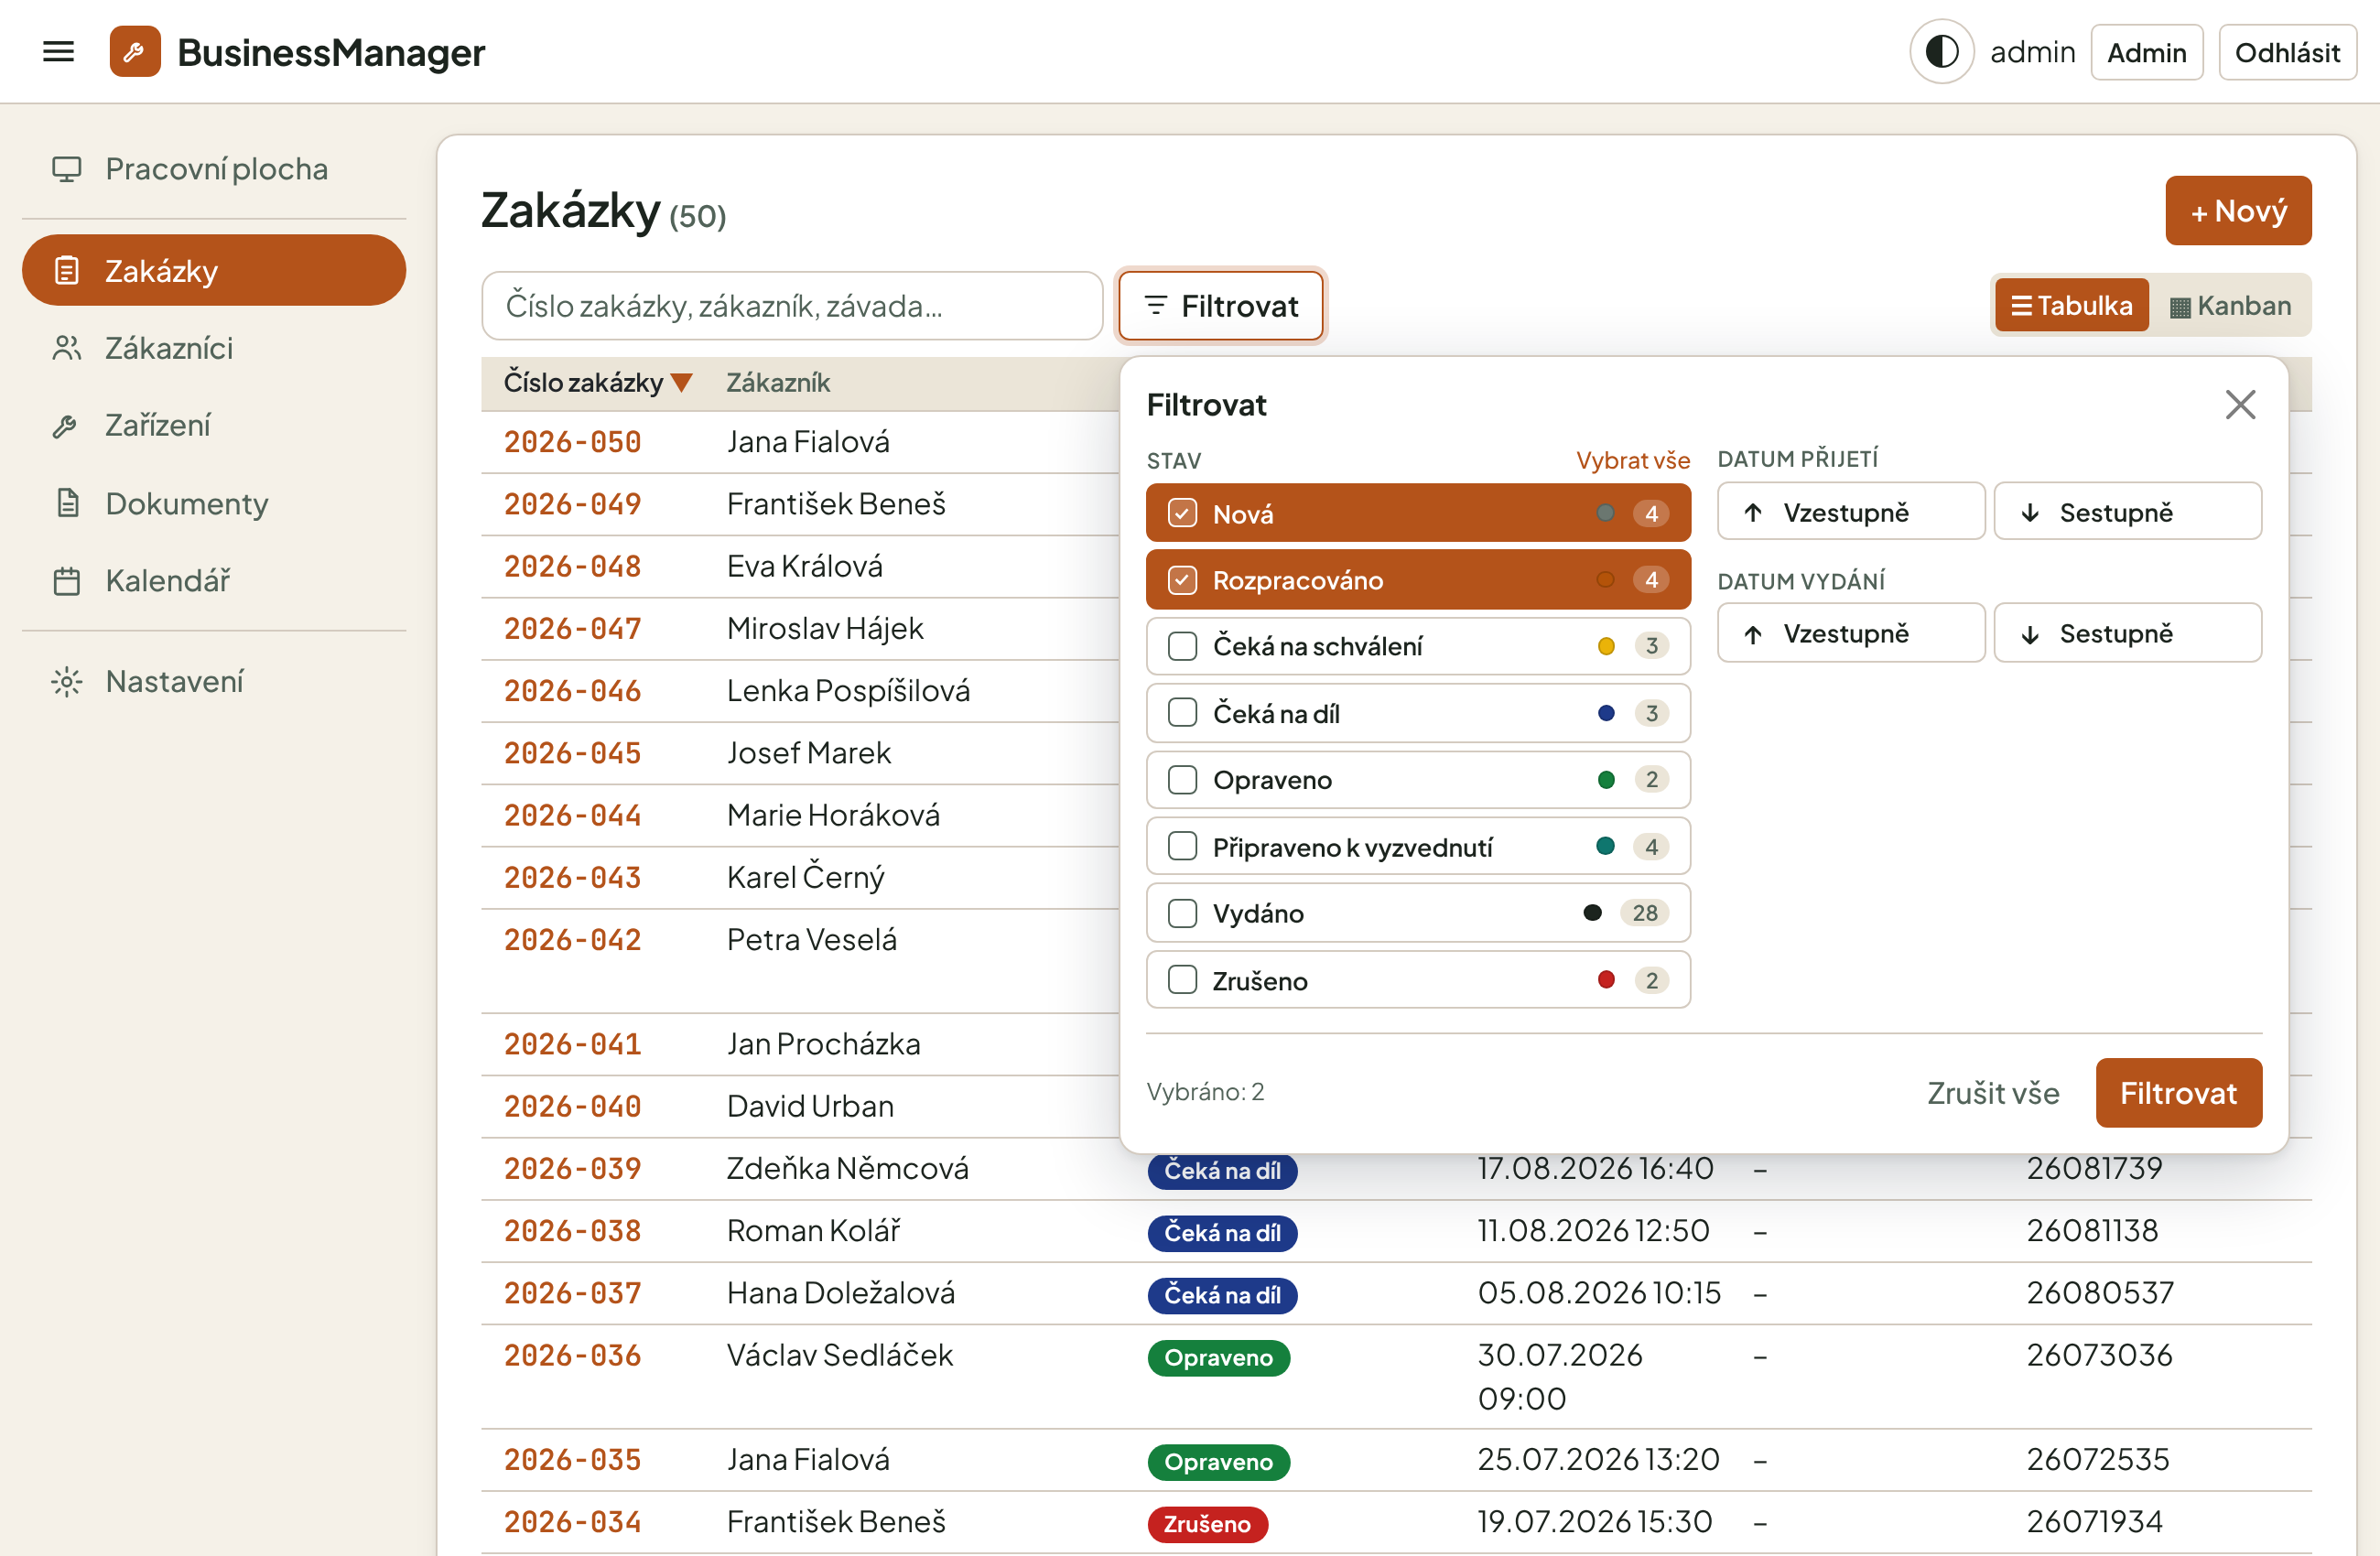
\includegraphics[width=\linewidth]{obrazky/navrh/bm-zakazky-filtr.png}
\caption{Seznam zakázek v~aplikaci s~otevřeným oknem Filtrovat, stavy s~počty záznamů a~řazením podle data (zdroj: vlastní)}\label{obr:bm-filtr-stavu}
\end{figure}

\begin{figure}[h]
\centering
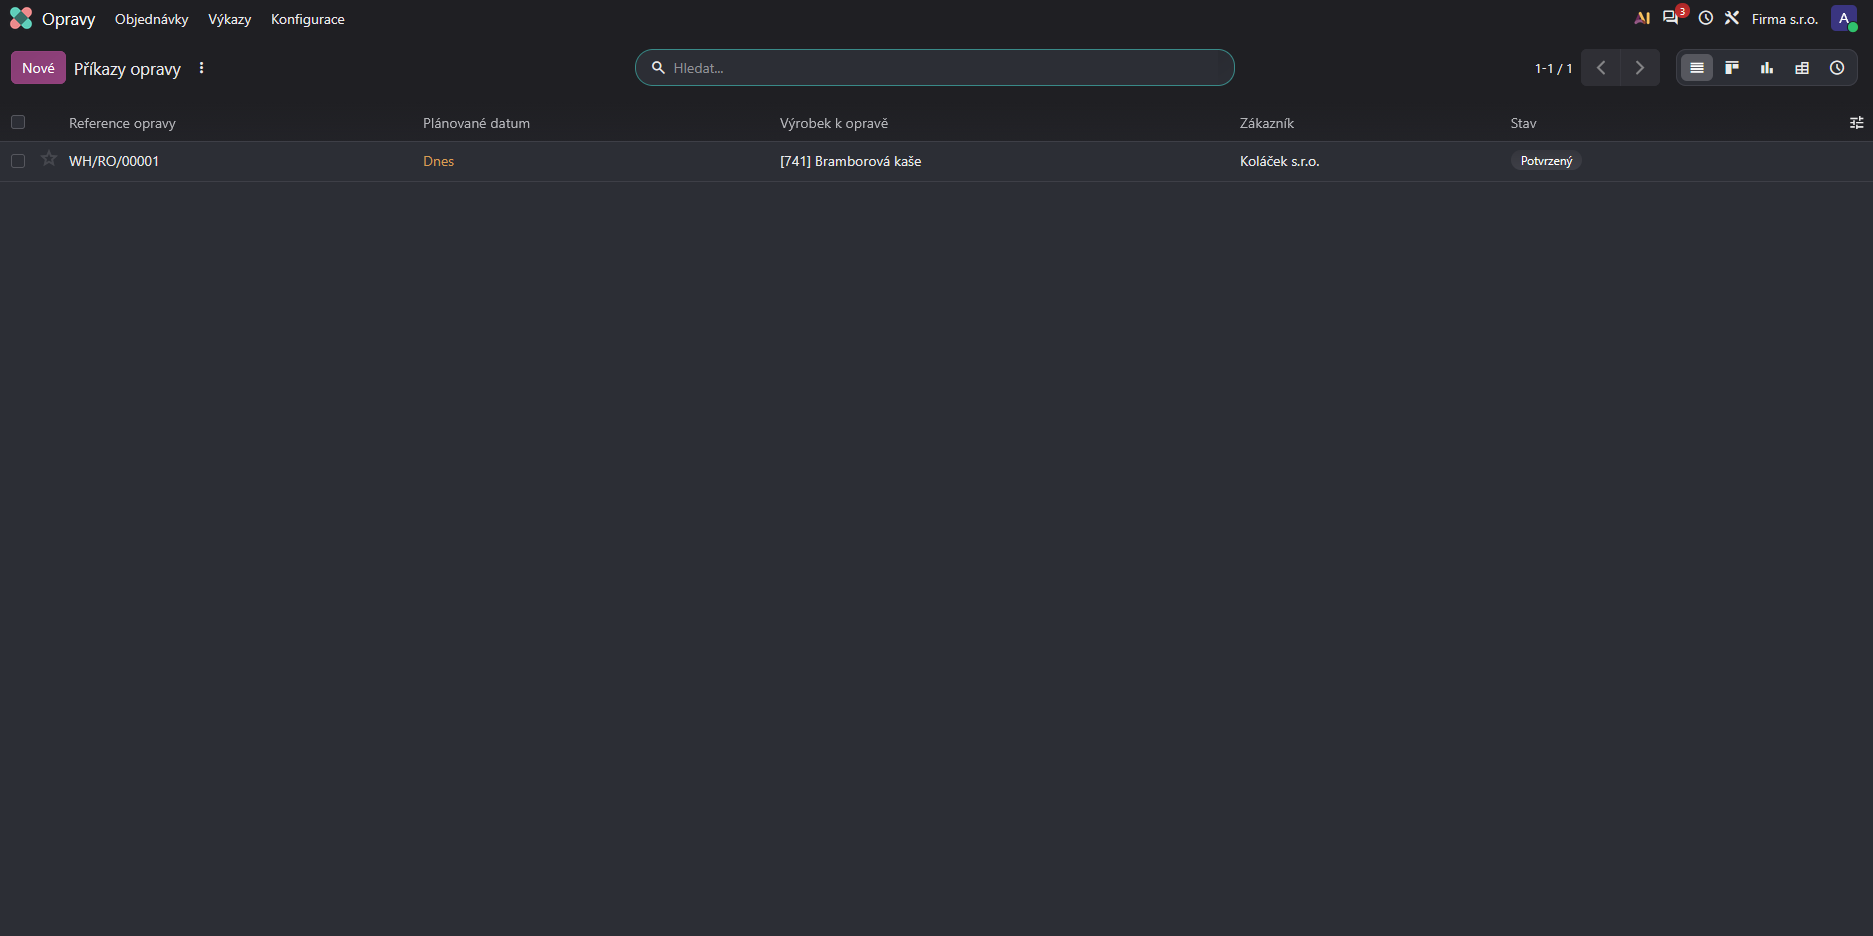
\includegraphics[width=\linewidth]{obrazky/reserse/odoo_strana_opravy.png}
\caption{Seznam oprav v~Odoo s~přepínačem zobrazení vpravo nahoře (seznam, kanban, graf, pivot, aktivity) (zdroj: vlastní snímek obrazovky ze zkušební verze, pořízeno 3.~11.~2026)}\label{obr:odoo-prepinac}
\end{figure}

\begin{figure}[h]
\centering
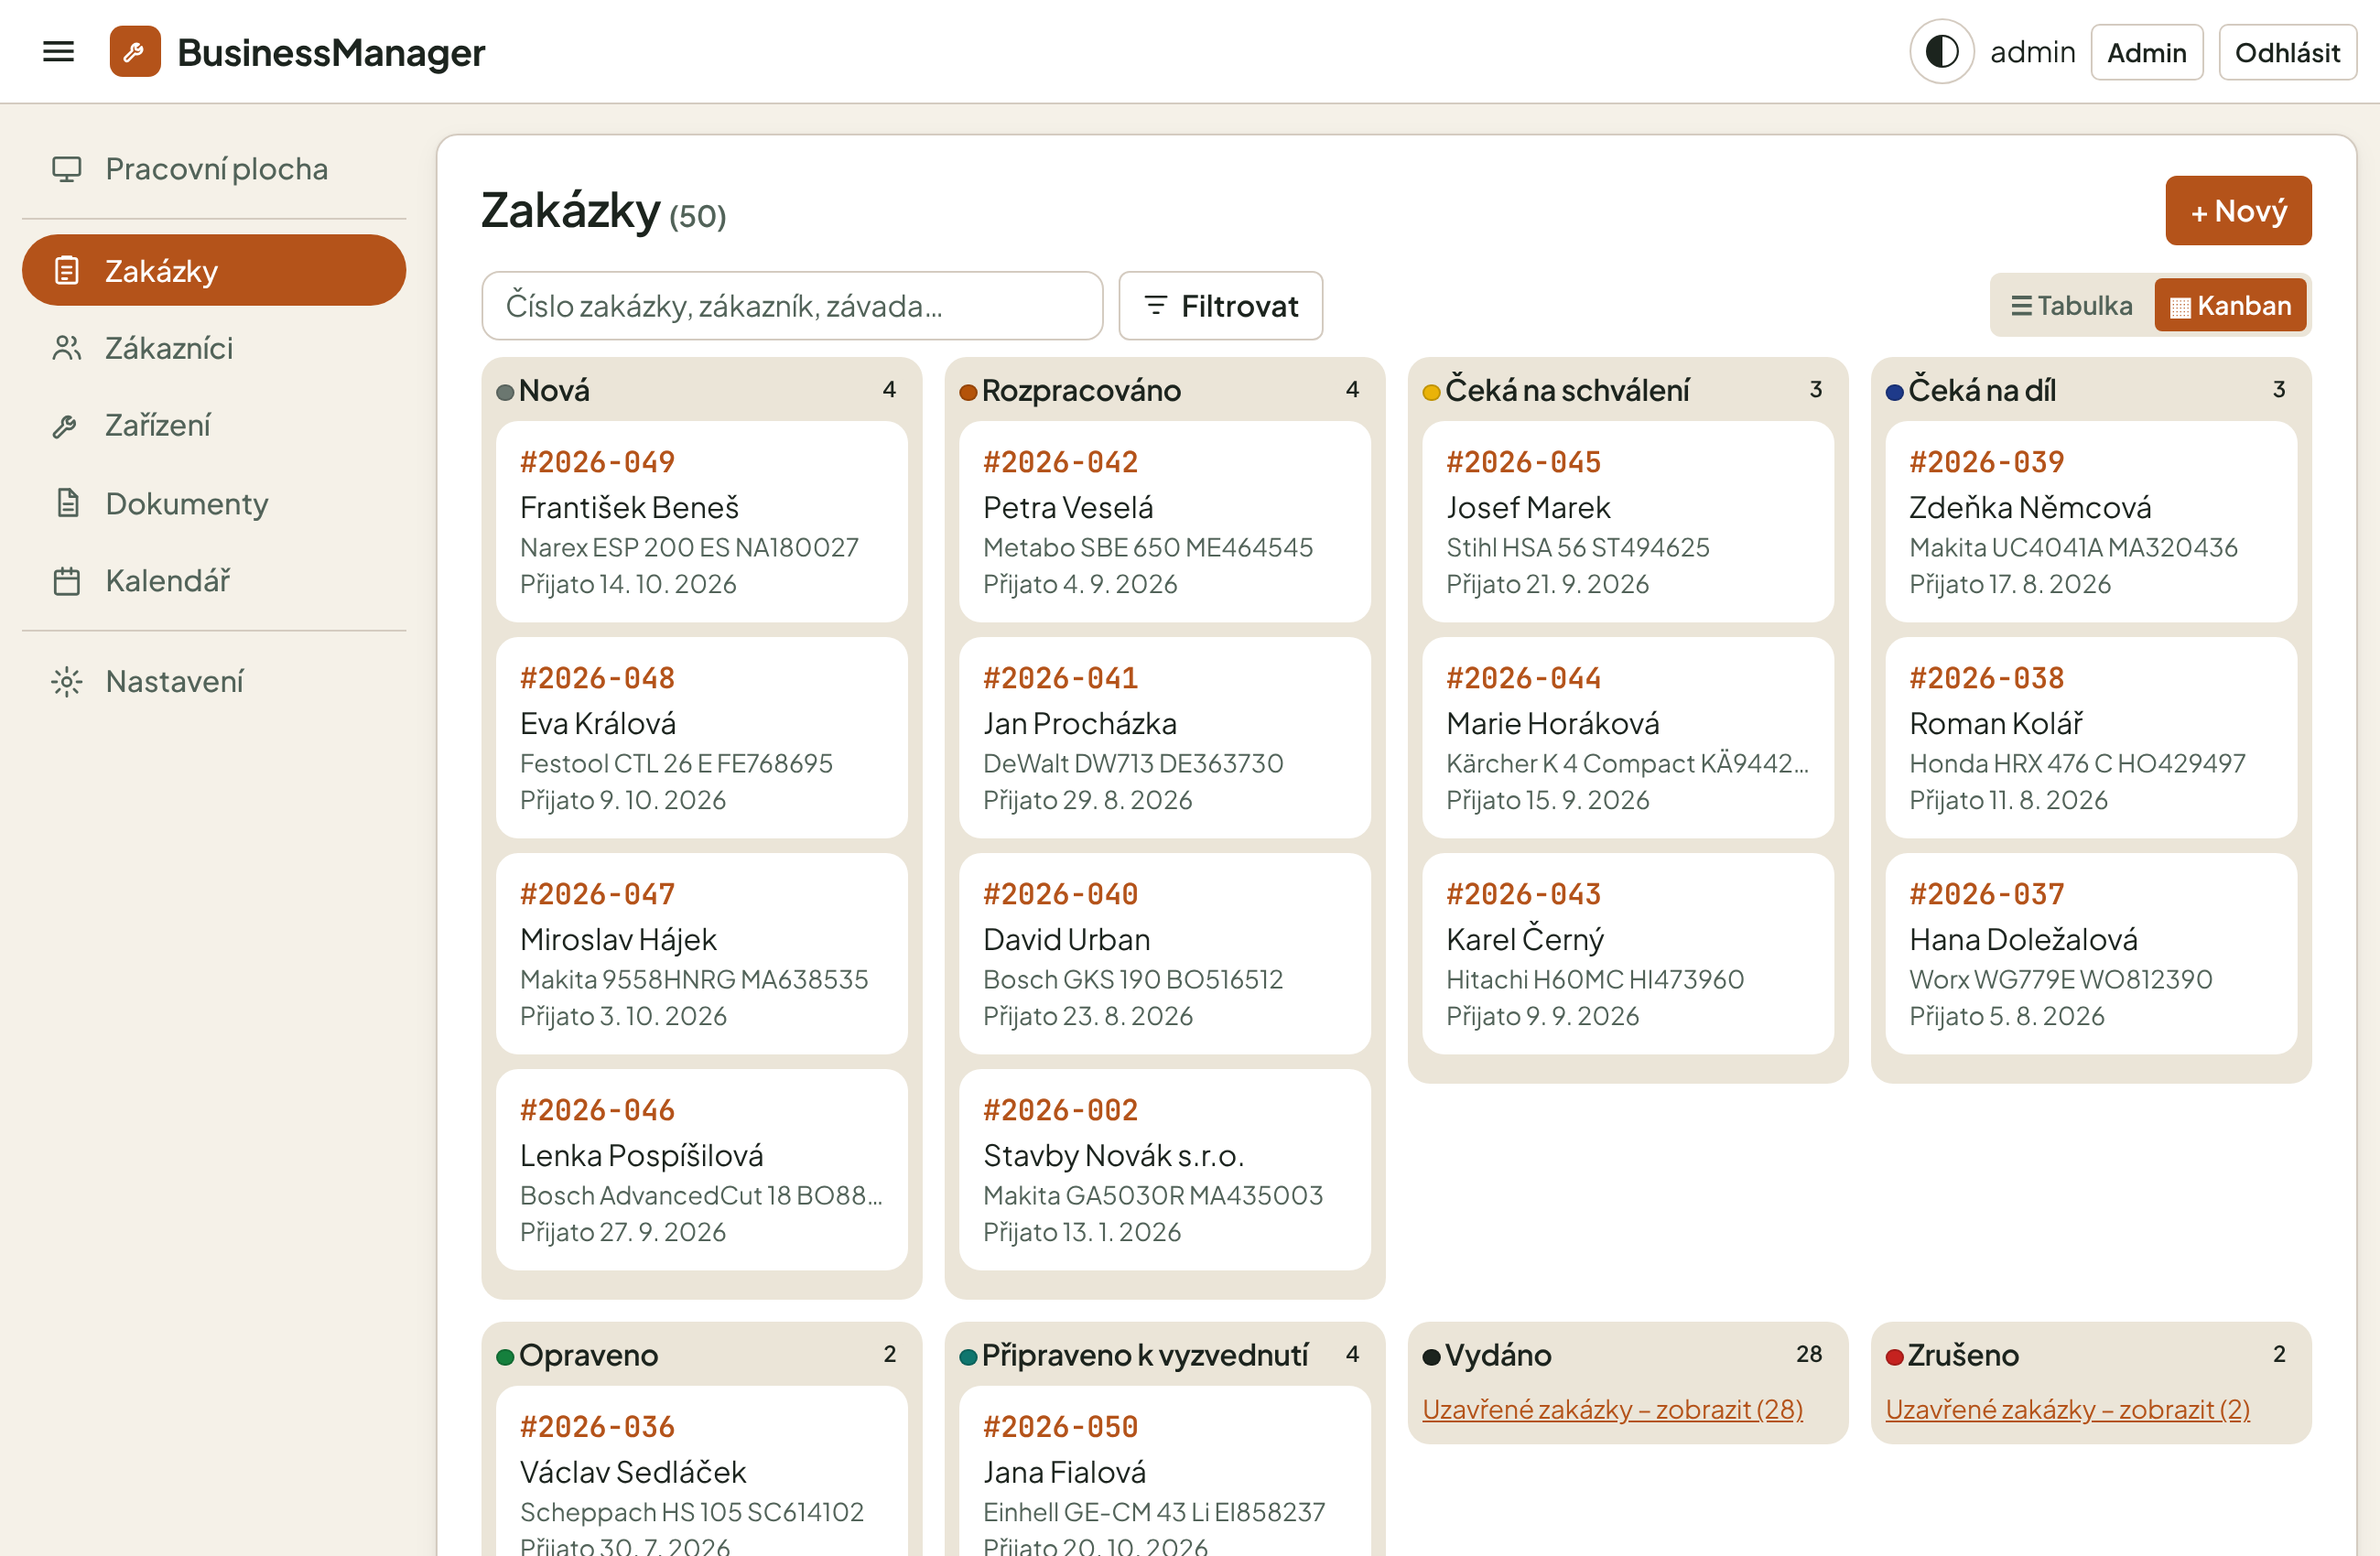
\includegraphics[width=\linewidth]{obrazky/navrh/bm-zakazky-kanban.png}
\caption{Kanbanové zobrazení zakázek v~aplikaci, sloupce odpovídají stavům zakázky, inspirováno Odoo (zdroj: vlastní)}\label{obr:bm-kanban}
\end{figure}

\subsection{Úpravy rozhraní podle doporučení}\label{sec:ui-upravy}

Při porovnání se zásadami vzniklo několik úprav a~všechny byly provedeny:
\begin{itemize}
\item Nastavení (údaje o~firmě, DPH, uživatelé, číselníky, šablony dokumentů, zálohování) bylo skryto a~zamčeno pro běžné zaměstnance. Později se rozdělení rozšířilo na role (Zaměstnanec, Technik, Administrativa, Administrátor): každý uživatel vidí jen tlačítka a~části aplikace, na které má oprávnění \cite{Nielsen-progressive}, \cite[s.~2331]{Sajedi2011}.
\item Styly Bootstrap a~knihovna htmx jsou přibaleny přímo do aplikace. Dříve se načítaly z~internetu a~bez připojení se aplikace zobrazila bez stylů, takže uživatel nevěděl, co se děje \cite{Nielsen-heuristiky}.
\item Při prvním spuštění provede aplikaci průvodce, který založí účet administrátora a~základní údaje o~firmě. Povinný je jen název organizace \cite{Nielsen-heuristiky}.
\item Na stránce zakázky bylo dříve osm stejně vypadajících tlačítek v~jedné řadě. Nyní zůstávají vpravo nahoře jen akce s~dokumenty (zakázkový list, nabídka, faktura, objednávka) a~tlačítka pro úpravu zakázky a~přidání práce, materiálu, fotografií a~příloh jsou v~záložkách, kterých se týkají. Plnou barvou je zvýrazněn jen doporučený další krok podle stavu zakázky, například zakázkový list u~nově přijaté zakázky, přidání práce u~rozpracované zakázky a~vytvoření nabídky a~poté faktury u~opravené zakázky. Je-li doporučeným krokem přidání práce, otevře se rovnou záložka Práce. Uživatel tak hned vidí, co má udělat dál \cite{Kaplan2021}, \cite{Shneiderman-pravidla}.
\item Na stránce zakázky byl dříve vpravo pevný panel prohlížeče dokumentů s~vlastní lištou tlačítek, který zabíral polovinu obrazovky i~tehdy, když uživatel žádný soubor neprohlížel. Nyní mají záložky celou šířku a~vejdou se do jedné řady. Fotografie, přílohy i~doklady se otevírají v~okně přes téměř celou obrazovku, ve kterém zůstalo jen stažení, tisk a~zavření, a~obrázek se přibližuje kolečkem myši. V~okně lze také porovnat dva soubory vedle sebe \cite{Nielsen-heuristiky}, \cite[s.~2332]{Sajedi2011}.
\item Údaje zařízení a~zákazníka se dříve upravovaly na samostatné stránce. Nyní tlačítko \enquote{Upravit} změní údaje přímo v~detailu na políčka a~tlačítka na \enquote{Uložit} a~\enquote{Zrušit}. Vedle údajů zařízení lze zobrazit fotografii nebo dokument z~jeho zakázek, například štítek s~typem a~sériovým číslem, takže je uživatel při přepisování nemusí držet v~paměti \cite{Shneiderman-pravidla}, \cite{Nielsen-heuristiky}.
\item Potvrzení nevratných akcí (například smazání) dříve zobrazoval systémový dialog prohlížeče s~adresou serveru. Nyní se zobrazí okno ve vzhledu aplikace se srozumitelnou otázkou a~tlačítkem, které říká, co se stane \cite{Shneiderman-pravidla}, \cite[s.~2331--2332]{Sajedi2011}.
\item Chybně zadaný e-mail nebo telefon dříve hlásila anglická bublina prohlížeče bez vysvětlení. Nyní formulář kontroluje server a~chybu ukáže česky u~políčka i~s~příkladem správného zápisu. Pole pro výběr souborů jsou také v~češtině \cite{Nielsen-heuristiky}.
\item Formuláře nové zakázky, nabídky a~faktury mají pod poli krátkou nápovědu, například že cena se zadává bez DPH a~DPH se dopočítá nebo že položky nabídky se převezmou ze zakázky \cite[s.~2330]{Sajedi2011}.
\end{itemize}

\endgroup
